\subsection{Behavioral Cloning}
\label{sec::322_bc}
Behavioral cloning in itself is not always related to machine learning, but poses one possible way of training a neural net in a supervised manner. The presented concept is easy to understand and got inspired by \cite{bojarski2016end}, where it was used for self-driving cars, and since having a car drive along the road is easier to achieve than having a robot walk around an environment, we will deal with the additional details later to focus on the main points for now. The proposed method utilizes the control loop, which was already introduced in figure \ref{fig::3_cl}. In order to then replace the human user by an artificial agent, we have a human user perform a desired behavior, and copy it. The required extended control loop is shown in figure \ref{fig::322_bc}.
\begin{figure}[h]
	\centering
	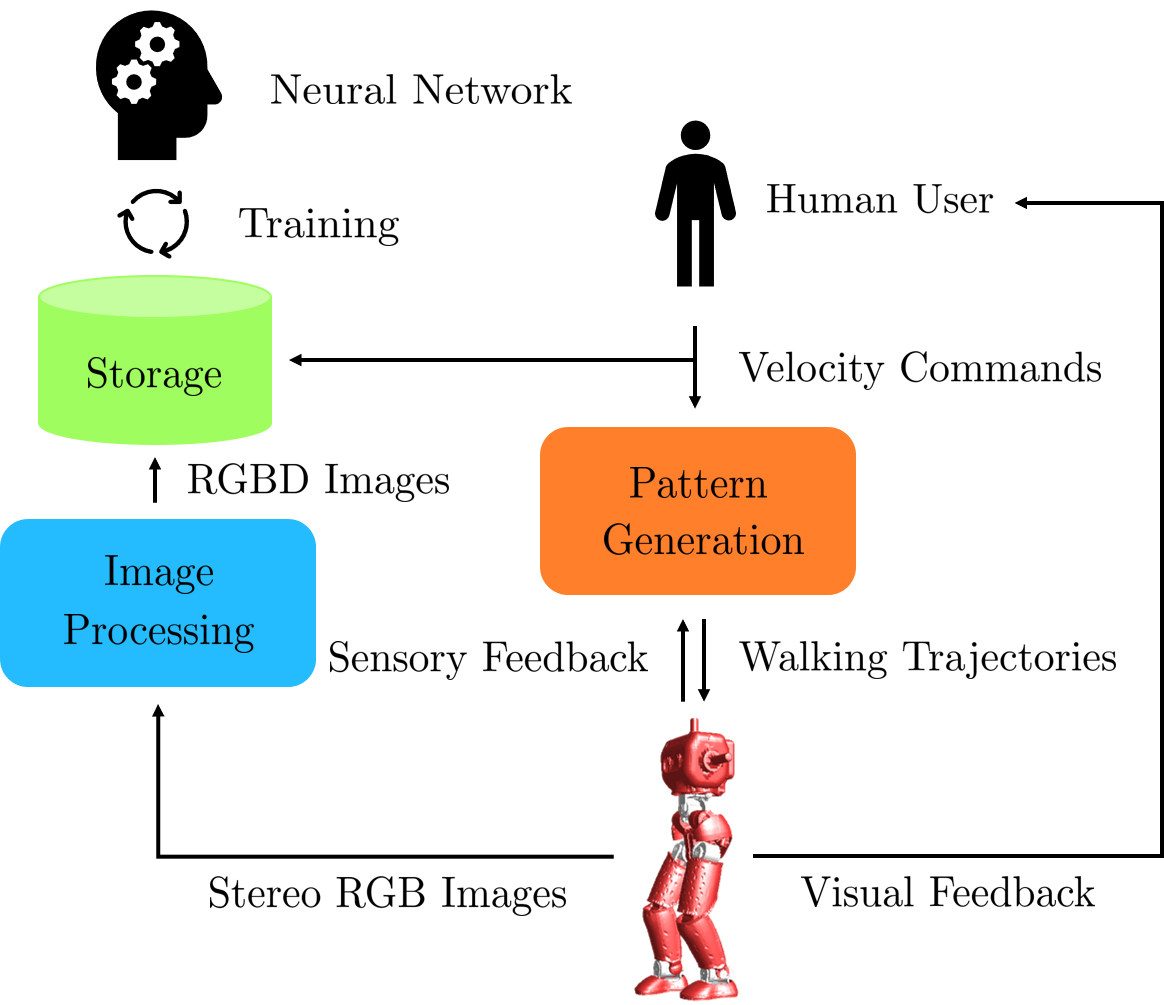
\includegraphics[scale=.5]{chapters/03_background/img/behavioral_cloning.png}
	\caption{Pipeline for behavioral cloning. The neural network is trained on stored RGBD images, and corresponding velocity commands that are correlated by a timestamp}
	\label{fig::322_bc}
\end{figure}
It simply takes the velocity commands from the human user, and stores it alongside RGBD images with a corresponding timestamp to some storage, where the RGBD images are obtained from stereo RGB images by an image processing step that is explained in section \ref{sec::324_ip}. The timestamp allows to correlate seen images to desired velocities afterwards, which in turn enables an artificial agent to train on the stored data. For our purposes, the artificial agent is a neural network. An appropriately chosen network architecture will then enable us to learn the taught behavior and ultimately lets us replace the human user. This procedure relies on prior knowledge to achieve certain tasks, namely the stored data. It is therefore extremely import to assure that the sampled data, from which we want to learn a task, does not introduce any unwanted bias, that is, we need to take care of the distribution from which we sample in the first place. In principle, it is possible to learn any arbitrary behavior with this technique, but this requires not only good data, but also a vast amount of it. There are other algorithms that explore the state space on their own, and for which we could for example use the taught behavior as prior as well. These algorithms belong to the class of reinforcement learning methods, and we will have a look at a particular one in the next section.